\documentclass[10pt,oneside,onecolumn,openany,final]{memoir}
\setstocksize{11in}{8.5in}

\usepackage[toc,lot,lof]{multitoc}
\usepackage[top=.5in, bottom=.5in, left=.75in, right=.75in]{geometry}
\usepackage{graphicx} \graphicspath{{./images/}}
\usepackage{longtable}
\usepackage{mdwlist}
\usepackage{microtype} \DisableLigatures{encoding = *, family = *}
\usepackage{multicol}
\usepackage{textcomp}
\usepackage[normalem]{ulem}
\usepackage{wrapfig}
\usepackage{xtab}
\usepackage{enumerate}
\usepackage{phonetic}
\usepackage{bbding}
\usepackage{linearb}
\usepackage{cypriot}
\usepackage{tipa}
\usepackage{xfrac}
\usepackage{appendix}
\usepackage{xparse}
\usepackage{letltxmacro}
\usepackage{makeidx} \makeindex
\usepackage[table,dvipsnames]{xcolor}
\definecolor{offyellow}{RGB}{255,255,128}
\definecolor{links}{RGB}{200,0,50}
\usepackage{placeins}
\usepackage{floatflt}
\usepackage{anyfontsize}

\usepackage[xcolor]{mdframed}
\usepackage{colortbl}
\usepackage{tabularx}

%% Font
\usepackage[T1]{fontenc}
\usepackage[bitstream-charter]{mathdesign}
\usepackage{aurical}

\usepackage[colorlinks=true,linkcolor=blue,urlcolor=links,pdfstartview={XYZ null null 1.00},bookmarksdepth=2]{hyperref}
%%%%%%%%%%%%%%%%%%%%%%%%%
%%%% End of Import tion %%%%%%%%%%%
%%%%%%%%%%%%%%%%%%%%%%%%%

%%%%%%%%%%%%%%%%%%%%%%%%%%%%%%%%%%%%%%%%%%%%%%%%%%
%%%%%%%%%%%%%%%%%%%%%%%%%%%%%%%%%%%%%%%%%%%%%%%%%%
%%% Revised Commands
%%%%%%%%%%%%%%%%%%%%%%%%%%%%%%%%%%%%%%%%%%%%%%%%%%
%%%%%%%%%%%%%%%%%%%%%%%%%%%%%%%%%%%%%%%%%%%%%%%%%%
\makeatletter

%fiddles with how chapter titles are displayed
\renewcommand{\@makechapterhead}[1]{%
\vspace*{0 pt}{%
\raggedright \normalfont \fontsize{32}{32} \selectfont \bfseries%
\ifnum \value{secnumdepth}>-1%
  \if@mainmatter \vspace{-8pt} {\fontsize{20}{20} \selectfont Chapter \thechapter:}\\[8pt]%
  \fi%
\fi
\hspace{0.65cm} #1\par\nobreak\vspace{20 pt}%
}}

%makes paragraphs show up closer together
\renewcommand{\paragraph}{%
\@startsection{paragraph}{4}%
{\z@}{1.0ex \@plus 1ex \@minus 0.2ex}{-1em} % wtf is an 'ex' anyways?
{\normalfont\normalsize\bfseries}%
}

%lets multicolumn have the proper background colors as defined by rowcolors
\let\oldmc\multicolumn
\newcommand{\mcinherit}{% Activate \multicolumn inheritance
  \renewcommand{\multicolumn}[3]{%
    \oldmc{##1}{##2}{\ifodd\rownum \@oddrowcolor\else\@evenrowcolor\fi ##3}%
  }}

\makeatother

%add labels within sections, subsections, and subsubsections
\LetLtxMacro{\oldsection}{\section}
\renewcommand{\section}[1]{\oldsection{#1}\label{sec:#1}}

\LetLtxMacro{\oldsubsection}{\subsection}
\renewcommand{\subsection}[1]{\oldsubsection{#1}\label{sec:#1}}

\LetLtxMacro{\oldsubsubsection}{\subsubsection}
\renewcommand{\subsubsection}[1]{\oldsubsubsection{#1}\label{sec:#1}}

%only put chapters and sections into the TOC
\setcounter{secnumdepth}{1}
%makes a subsubsection start off indented.
\setlength{\beforesubsubsecskip}{-\beforesubsubsecskip}

%%%%%%%%%%%%%%%%%%%%%%%%%%%%%%%%%%%%%%%%%%%%%%%%%%
%%%%%%%%%%%%%%%%%%%%%%%%%%%%%%%%%%%%%%%%%%%%%%%%%%
%%% Table Formatting
%%%%%%%%%%%%%%%%%%%%%%%%%%%%%%%%%%%%%%%%%%%%%%%%%%
%%%%%%%%%%%%%%%%%%%%%%%%%%%%%%%%%%%%%%%%%%%%%%%%%%
\newcolumntype{L}[1]{>{\raggedright\let\newline\\\arraybackslash\hspace{0pt}}m{#1}} %New type of column 'L' that is ragged-right, behaves like a paragraph, and allows manual definition of width like a 'p' column.
\newcolumntype{C}[1]{>{\centering\let\newline\\\arraybackslash\hspace{0pt}}m{#1}}  %New type of column 'C' that is centered, behaves like a paragraph, and allows manual definition of width like a 'p' column.
\newcolumntype{R}[1]{>{\raggedleft\let\newline\\\arraybackslash\hspace{0pt}}m{#1}}  %New type of column 'R' that is ragged-left, behaves like a paragraph, and allows manual definition of width like a 'p' column.
\newcommand{\startclasstable}{
	\begin{table}[htb]
	\centering
	\begin{small}
	\rowcolors{1}{colorone}{colortwo}}
%sets up the basic formatting for class entry tables without needing manual entry. Just place the tabular after this.
\newcommand{\stopclasstable}{
	\end{small}
	\end{table}}
%twin of \classtable, ends the small and table environments, place after \end{tabular}
\newcommand{\header}{\rowcolor{headercolor}}
%when inserted in a row, makes that row the color headercolor

%%%%%%%%%%%%%%%%%%%%%%%%%%%%%%%%%%%%%%%%%%%%%%%%%%
%%%%%%%%%%%%%%%%%%%%%%%%%%%%%%%%%%%%%%%%%%%%%%%%%%
%%% New Commands
%%%%%%%%%%%%%%%%%%%%%%%%%%%%%%%%%%%%%%%%%%%%%%%%%%
%%%%%%%%%%%%%%%%%%%%%%%%%%%%%%%%%%%%%%%%%%%%%%%%%%

%%%%%%%%%%%%%%%%%%%%%%%%
%%Basic Formatting
%%%%%%%%%%%%%%%%%%%%%%%%
\newcommand{\originallineskip}{\baselineskip}
 %A command that is equal to the original \baselineskip of the doc, in case we change it for a section and want to change it back later
\newmdenv[hidealllines=true,backgroundcolor=gray!20]{abilitybox}
%A new environemnt, abilty box, that gets redefined by other commands later, notably to produce color backgrounds for classes
\newcommand{\ability}[2]{\smallskip \noindent \textbf{#1} #2} 
%The \ability{#1}{#2} command from legacy-source. Should rarely be directly used, changes to this will cascade into other new commands that use its functionality
\newcommand{\itemspace}{\setlength{\itemsep}{-1mm}\setlength{\topsep}{-1mm} }
%A command from legacy-source for compatabilty
\newcommand{\listone}{\begin{list}{$\bullet$}{\itemspace}}
%A type of list from legacy sorce
\newcommand{\spell}[1]{\emph{\MakeLowercase{#1}}}
%makes spell name lowercase italics.

%%%%%%%%%%%%%%%%%%%%%%%%
%%Logic
%%%%%%%%%%%%%%%%%%%%%%%%
\newcommand{\testempty}{\empty}
\newcommand{\isempty}{\empty}
%Two commands that can be compared to one another for \ifx logic tests. \isempty should never be changed. If \testempty holds a value of anything but empty, the test should return false.
\newcommand{\zero}{0}
\newcommand{\one}{1}
\newcommand{\two}{2}
\newcommand{\three}{3}
\newcommand{\four}{4}
\newcommand{\five}{5}
\newcommand{\six}{6}
\newcommand{\seven}{7}
\newcommand{\eight}{8}
\newcommand{\nine}{9}

%%%%%%%%%%%%%%%%%%%%%%%%
%%Colors
%%%%%%%%%%%%%%%%%%%%%%%%
\colorlet{colorone}{white}
\colorlet{colortwo}{gray!15}
\colorlet{headercolor}{gray!50}
\colorlet{tablecolorone}{gray!40}
\colorlet{tablecolortwo}{gray!20}

%%%%%%%%%%%%%%%%%%%%%%%%
%%Sectioning
%%%%%%%%%%%%%%%%%%%%%%%%
\newcommand{\classentry}[1]{\newpage \section{#1} \renewcommand{\class}{#1} \index{#1 (class)} \renewcommand{\testempty}{\empty}}
%Starts a new page, creates a section with the name of the class (#1), sets \class to be the name of the class, indexes the class.
\newcommand{\raceentry}[1]{\oldsection{#1}\index{#1 (race)}\label{race:#1}}

\newcommand{\Requirements}{\oldsubsubsection*{Requirements}}

\newcommand{\Basics}{\oldsubsubsection*{Basics}}

\newcommand{\ClassFeatures}{\oldsubsubsection*{Class Features}}

\newcommand{\skillentry}[2]{\oldsubsection[#1]{#1 #2}\index{#1 (skill)}\label{skill:#1}}

%%%%%%%%%%%%%%%%%%%%%%%%
%%Class Chapter
%%%%%%%%%%%%%%%%%%%%%%%%
\newcommand{\class}{placeholder}
%Holds the classes name, as defined by \classentry

\newcommand{\quot}[1]{
	\vspace{-8pt}
	\noindent\emph{#1}\medskip}
%Displays a flavor quote.}

\newcommand{\desc}[1]{
  \ifx\testempty\isempty\renewmdenv[hidealllines=true,backgroundcolor=colorone]{abilitybox}\renewcommand{\testempty}{a}\else\renewcommand{\testempty}{\empty}\renewmdenv[hidealllines=true,backgroundcolor=colortwo]{abilitybox}\fi
\begin{abilitybox}#1 \medskip\end{abilitybox}}
%Places descriptive text for class in an abilitybox environment and colors it automatically based on colorone and colortwo. Implimentation looks like \desc{Text text text text etc.}

\newcommand{\playingaclass}[1]{
  \ifx\testempty\isempty\renewmdenv[hidealllines=true,backgroundcolor=colorone]{abilitybox}\renewcommand{\testempty}{a}\else\renewcommand{\testempty}{\empty}\renewmdenv[hidealllines=true,backgroundcolor=colortwo]{abilitybox}\fi
  \begin{abilitybox}\ability{Playing a \class :}{#1}\end{abilitybox}}
%Places the "playing a CLASS" text for class in an abilitybox environment and colors it automatically based on colorone and colortwo. Reliant on \ability command. Implimentaion looks like \playingaclass{how to play the class}

\newcommand{\hitdie}[1]{
  \ifx\testempty\isempty\renewmdenv[hidealllines=true,backgroundcolor=colorone]{abilitybox}\renewcommand{\testempty}{a}\else\renewcommand{\testempty}{\empty}\renewmdenv[hidealllines=true,backgroundcolor=colortwo]{abilitybox}\fi
  \begin{abilitybox}\ability{Hit Die:}{#1}\end{abilitybox}}
%Places hit die text for class in an abilitybox environment and colors it automatically based on colorone and colortwo. Reliant on \ability command. Implimentaion looks like \hitdie{d#}

\newcommand{\alignment}[1]{
  \ifx\testempty\isempty\renewmdenv[hidealllines=true,backgroundcolor=colorone]{abilitybox}\renewcommand{\testempty}{a}\else\renewcommand{\testempty}{\empty}\renewmdenv[hidealllines=true,backgroundcolor=colortwo]{abilitybox}\fi
  \begin{abilitybox}\ability{Alignment:}{#1}\end{abilitybox}}
%Places alignment requirement for class in an abilitybox environment and colors it automatically based on colorone and colortwo. Implimentation looks like \alignment{chosen alignment(s)}

\newcommand{\races}[1]{
  \ifx\testempty\isempty\renewmdenv[hidealllines=true,backgroundcolor=colorone]{abilitybox}\renewcommand{\testempty}{a}\else\renewcommand{\testempty}{\empty}\renewmdenv[hidealllines=true,backgroundcolor=colortwo]{abilitybox}\fi
  \begin{abilitybox}\ability{Races:}{#1}\end{abilitybox}}
%Places races requirement for class in an abilitybox environment and colors it automatically based on colorone and colortwo. Implimentation looks like \races{List of races}

\newcommand{\startinggold}[1]{
  \ifx\testempty\isempty\renewmdenv[hidealllines=true,backgroundcolor=colorone]{abilitybox}\renewcommand{\testempty}{a}\else\renewcommand{\testempty}{\empty}\renewmdenv[hidealllines=true,backgroundcolor=colortwo]{abilitybox}\fi
  \begin{abilitybox}\ability{Starting Gold:}{#1}\end{abilitybox}}
%Places starting gold for class in an abilitybox environment and colors it automatically based on colorone and colortwo. Implimentation looks like \startinggold{#d#}

\newcommand{\startingage}[1]{
  \ifx\testempty\isempty\renewmdenv[hidealllines=true,backgroundcolor=colorone]{abilitybox}\renewcommand{\testempty}{a}\else\renewcommand{\testempty}{\empty}\renewmdenv[hidealllines=true,backgroundcolor=colortwo]{abilitybox}\fi
  \begin{abilitybox}\ability{Starting Age:}{#1}\end{abilitybox}}  
%Places starting age for class in an abilitybox environment and colors it automatically based on colorone and colortwo. Implimentation looks like \startingage{age at which you start}

\newcommand{\skillpoints}[1]{
  \ifx\testempty\isempty\renewmdenv[hidealllines=true,backgroundcolor=colorone]{abilitybox}\renewcommand{\testempty}{a}\else\renewcommand{\testempty}{\empty}\renewmdenv[hidealllines=true,backgroundcolor=colortwo]{abilitybox}\fi
  \begin{abilitybox}\ability{Skill Points per Level:}{#1 + Intelligence Bonus}\end{abilitybox}}
%Places skill points gained per level for class in an abilitybox environment and colors it automatically based on colorone and colortwo. Implimentation looks like \skillpoints{#}

\newcommand{\classskills}[1]{
  \ifx\testempty\isempty\renewmdenv[hidealllines=true,backgroundcolor=colorone]{abilitybox}\renewcommand{\testempty}{a}\else\renewcommand{\testempty}{\empty}\renewmdenv[hidealllines=true,backgroundcolor=colortwo]{abilitybox}\fi
  \begin{abilitybox}\ability{Class Skills:}{The {\class}'s class skills (and the key ability for each skill) are #1}\end{abilitybox}}
%Places class skills for class in an abilitybox environment and colors it automatically based on colorone and colortwo. Implimentation looks like \classskills{Skill (Key Ability), Skill Two (Key Ability), and Etc. (etc)}

\newcommand{\startclassfeatures}{
 \smallskip\noindent All of the following are class features of the \class ~class.}
%place before actual class features entries.

\newcommand{\proficiencies}[1]{
 \ability{Weapon and Armor Proficiencies:}{The \class ~is proficient with #1}}
%Displays proficiencies with minimal input, implimentation looks like \proficiencies{the proficiencies}

\newcommand{\classfeature}[2]{
  \ability{#1}{#2}}
%No functional difference from \ability currently

%%%%Class Table Commands

\newcommand{\gbab}{\empty}
\newcommand{\mbab}{\empty}
\newcommand{\fort}{\empty}
\newcommand{\refl}{\empty}
\newcommand{\will}{\empty}
%Creates new commands for use in \ifx statements for formatting purposes.

\newcommand{\goodbab}{\renewcommand{\gbab}{\empty}\renewcommand{\mbab}{a}}
\newcommand{\modebab}{\renewcommand{\gbab}{a}\renewcommand{\mbab}{\empty}}
\newcommand{\poorbab}{\renewcommand{\gbab}{a}\renewcommand{\mbab}{a}}
%A set of commands to tell LaTeX what BAB progression the class has. Only one should be called per class.

\newcommand{\goodfor}{\renewcommand{\fort}{\empty}}
\newcommand{\poorfor}{\renewcommand{\fort}{a}}
%A set of commands to tell LaTeX what Fortitude progression the class has. Only one should be called per class.

\newcommand{\goodref}{\renewcommand{\refl}{\empty}}
\newcommand{\poorref}{\renewcommand{\refl}{a}}
%A set of commands to tell LaTeX what Reflex progression the class has. Only one should be called per class.

\newcommand{\goodwil}{\renewcommand{\will}{\empty}}
\newcommand{\poorwil}{\renewcommand{\will}{a}}
%A set of commands to tell LaTeX what Will progression the class has. Only one should be called per class.

\newenvironment{classtable}[1]
{
\table[htb]
\center
\rowcolors{1}{colorone}{colortwo}
\tabularx{\textwidth}{p{.275in}p{.75in}p{0.275in}p{0.275in}p{0.275in}Xllll}
\rowcolor{gray!50} Level & Base Attack & fort. & Ref. & Will & Special #1\\
}{
\endtabularx
\endcenter
\endtable
}

%A a new environment that sets up the class tables. Include the \level commands between \begin{classtable}.

\newcommand{\levelone}[1]{
1st  & \ifx\gbab\isempty +1 \else\ifx\mbab\isempty +0 \else +0 \fi \fi
	 & \ifx\fort\isempty +2 \else +0 \fi
	 & \ifx\refl\isempty +2 \else +0 \fi
	 & \ifx\will\isempty +2 \else +0 \fi
	 & #1 \\}
%A command that declares a table row within the class feature table.

\newcommand{\leveltwo}[1]{
2nd  & \ifx\gbab\isempty +2 \else\ifx\mbab\isempty +1 \else +1 \fi \fi
	 & \ifx\fort\isempty +3 \else +0 \fi
	 & \ifx\refl\isempty +3 \else +0 \fi
	 & \ifx\will\isempty +3 \else +0 \fi
	 & #1 \\}
%A command that declares a table row within the class feature table.

\newcommand{\levelthree}[1]{
3rd  & \ifx\gbab\isempty +3 \else\ifx\mbab\isempty +2 \else +1 \fi \fi
	 & \ifx\fort\isempty +3 \else +1 \fi
	 & \ifx\refl\isempty +3 \else +1 \fi
	 & \ifx\will\isempty +3 \else +1 \fi
	 & #1 \\}
%A command that declares a table row within the class feature table.

\newcommand{\levelfour}[1]{
4th  & \ifx\gbab\isempty +4 \else\ifx\mbab\isempty +3 \else +2 \fi \fi
	 & \ifx\fort\isempty +4 \else +1 \fi
	 & \ifx\refl\isempty +4 \else +1 \fi
	 & \ifx\will\isempty +4 \else +1 \fi
	 & #1 \\}
%A command that declares a table row within the class feature table.

\newcommand{\levelfive}[1]{
5th  & \ifx\gbab\isempty +5 \else\ifx\mbab\isempty +3 \else +2 \fi \fi
	 & \ifx\fort\isempty +4 \else +1 \fi
	 & \ifx\refl\isempty +4 \else +1 \fi
	 & \ifx\will\isempty +4 \else +1 \fi
	 & #1 \\}
%A command that declares a table row within the class feature table.
	 
\newcommand{\levelsix}[1]{
6th  & \ifx\gbab\isempty +6/+1 \else\ifx\mbab\isempty +4 \else +3 \fi \fi
	 & \ifx\fort\isempty +5 \else +2 \fi
	 & \ifx\refl\isempty +5 \else +2 \fi
	 & \ifx\will\isempty +5 \else +2 \fi
	 & #1 \\}
%A command that declares a table row within the class feature table.

\newcommand{\levelseven}[1]{
7th  & \ifx\gbab\isempty +7/+2 \else\ifx\mbab\isempty +5 \else +3 \fi \fi
	 & \ifx\fort\isempty +5 \else +2 \fi
	 & \ifx\refl\isempty +5 \else +2 \fi
	 & \ifx\will\isempty +5 \else +2 \fi
	 & #1 \\}
%A command that declares a table row within the class feature table.
	 
\newcommand{\leveleight}[1]{
8th  & \ifx\gbab\isempty +8/+3 \else\ifx\mbab\isempty +6/+1 \else +4 \fi \fi
	 & \ifx\fort\isempty +6 \else +2 \fi
	 & \ifx\refl\isempty +6 \else +2 \fi
	 & \ifx\will\isempty +6 \else +2 \fi
	 & #1 \\}
%A command that declares a table row within the class feature table.
	 
\newcommand{\levelnine}[1]{
9th  & \ifx\gbab\isempty +9/+4 \else\ifx\mbab\isempty +6/+1 \else +4 \fi \fi
	 & \ifx\fort\isempty +6 \else +3 \fi
	 & \ifx\refl\isempty +6 \else +3 \fi
	 & \ifx\will\isempty +6 \else +3 \fi
	 & #1 \\}
%A command that declares a table row within the class feature table.
	 
\newcommand{\levelten}[1]{
10th & \ifx\gbab\isempty +10/+5 \else\ifx\mbab\isempty +7/+2 \else +5 \fi \fi
	 & \ifx\fort\isempty +7 \else +3 \fi
	 & \ifx\refl\isempty +7 \else +3 \fi
	 & \ifx\will\isempty +7 \else +3 \fi
	 & #1 \\}
%A command that declares a table row within the class feature table.
	 
\newcommand{\leveleleven}[1]{
11th & \ifx\gbab\isempty +11/+6/+6 \else\ifx\mbab\isempty +8/+3 \else +5 \fi \fi
	 & \ifx\fort\isempty +7 \else +3 \fi
	 & \ifx\refl\isempty +7 \else +3 \fi
	 & \ifx\will\isempty +7 \else +3 \fi
	 & #1 \\}
%A command that declares a table row within the class feature table.
	 
\newcommand{\leveltwelve}[1]{
12th & \ifx\gbab\isempty +12/+7/+7 \else\ifx\mbab\isempty +9/+4 \else +6/+1 \fi \fi
	 & \ifx\fort\isempty +8 \else +4 \fi
	 & \ifx\refl\isempty +8 \else +4 \fi
	 & \ifx\will\isempty +8 \else +4 \fi
	 & #1 \\}
%A command that declares a table row within the class feature table.
	 
\newcommand{\levelthirteen}[1]{
13th & \ifx\gbab\isempty +13/+8/+8 \else\ifx\mbab\isempty +9/+4 \else +6/+1 \fi \fi
	 & \ifx\fort\isempty +8 \else +4 \fi
	 & \ifx\refl\isempty +8 \else +4 \fi
	 & \ifx\will\isempty +8 \else +4 \fi
	 & #1 \\}
%A command that declares a table row within the class feature table.
	 
\newcommand{\levelfourteen}[1]{
14th & \ifx\gbab\isempty +14/+9/+9 \else\ifx\mbab\isempty +10/+5 \else +7/+2 \fi \fi
	 & \ifx\fort\isempty +9 \else +4 \fi
	 & \ifx\refl\isempty +9 \else +4 \fi
	 & \ifx\will\isempty +9 \else +4 \fi
	 & #1 \\}
%A command that declares a table row within the class feature table.
	 
\newcommand{\levelfifteen}[1]{
15th & \ifx\gbab\isempty +15/+10/+10 \else\ifx\mbab\isempty +11/+6/+6 \else +7/+2 \fi \fi
	 & \ifx\fort\isempty +9 \else +5 \fi
	 & \ifx\refl\isempty +9 \else +5 \fi
	 & \ifx\will\isempty +9 \else +5 \fi
	 & #1 \\}
%A command that declares a table row within the class feature table.
	 
\newcommand{\levelsixteen}[1]{
16th & \ifx\gbab\isempty +16/+11/+11/+11 \else\ifx\mbab\isempty +12/+7/+7 \else +8/+3 \fi \fi
	 & \ifx\fort\isempty +10 \else +5 \fi
	 & \ifx\refl\isempty +10 \else +5 \fi
	 & \ifx\will\isempty +10 \else +5 \fi
	 & #1 \\}
%A command that declares a table row within the class feature table.
	 
\newcommand{\levelseventeen}[1]{
17th & \ifx\gbab\isempty +17/+12/+12/+12 \else\ifx\mbab\isempty +12/+7/+7 \else +8/+3 \fi \fi
	 & \ifx\fort\isempty +10 \else +5 \fi
	 & \ifx\refl\isempty +10 \else +5 \fi
	 & \ifx\will\isempty +10 \else +5 \fi
	 & #1 \\}
%A command that declares a table row within the class feature table.
	 
\newcommand{\leveleighteen}[1]{
18th & \ifx\gbab\isempty +18/+13/+13/+13 \else\ifx\mbab\isempty +13/+8/+8 \else +9/+4 \fi \fi
	 & \ifx\fort\isempty +11 \else +6 \fi
	 & \ifx\refl\isempty +11 \else +6 \fi
	 & \ifx\will\isempty +11 \else +6 \fi
	 & #1 \\}
%A command that declares a table row within the class feature table.
	 
\newcommand{\levelnineteen}[1]{
19th & \ifx\gbab\isempty +19/+14/+14/+14 \else\ifx\mbab\isempty +14/+9/+9 \else +9/+4 \fi \fi
	 & \ifx\fort\isempty +11 \else +6 \fi
	 & \ifx\refl\isempty +11 \else +6 \fi
	 & \ifx\will\isempty +11 \else +6 \fi
	 & #1 \\}
%A command that declares a table row within the class feature table.
	 
\newcommand{\leveltwenty}[1]{
20th & \ifx\gbab\isempty +20/+15/+15/+15 \else\ifx\mbab\isempty +15/+10/+10 \else +10/+5 \fi \fi
	 & \ifx\fort\isempty +12 \else +6 \fi
	 & \ifx\refl\isempty +12 \else +6 \fi
	 & \ifx\will\isempty +12 \else +6 \fi
	 & #1 \\}
%A command that declares a table row within the class feature table.

%%%%%%%%%%%%%%%%%%%%%%%%
%%Unsorted Commands
%%%%%%%%%%%%%%%%%%%%%%%%
\newcommand{\tagline}[1]{\vspace{-6pt} \textit{#1} \medskip}

\newcommand{\gameterm}[1]{#1\index{#1}}

\NewDocumentCommand\featentry{m+g}{%
  \IfNoValueTF{#2}
    {\oldsubsubsection[#1]{#1 [General]}\label{feat:#1}}%no second arg, general feat
    {\oldsubsubsection[#1]{#1 [#2]}\label{feat:#1}}%second arg, special type of feat
}

\newcommand{\spellentry}[1]{\oldsubsubsection{#1}\label{spell:#1}}

\NewDocumentCommand\linkrace{m+g}{%
  \IfNoValueTF{#2}
    {\hyperref[race:#1]{#1}}%no second arg, display is same as link
    {\hyperref[race:#1]{#2}}%second arg, link to first and display second
}
\NewDocumentCommand\linkclass{m+g}{%
  \IfNoValueTF{#2}
    {\hyperref[class:#1]{#1}}%no second arg, display is same as link
    {\hyperref[class:#1]{#2}}%second arg, link to first and display second
}
\NewDocumentCommand\linkskill{m+g}{%
  \IfNoValueTF{#2}
    {\hyperref[skill:#1]{#1}}%no second arg, display is same as link
    {\hyperref[skill:#1]{#2}}%second arg, link to first and display second
}
\NewDocumentCommand\linkfeat{m+g}{%
  \IfNoValueTF{#2}
    {\hyperref[feat:#1]{#1}}%no second arg, display is same as link
    {\hyperref[feat:#1]{#2}}%second arg, link to first and display second
}
\NewDocumentCommand\linkspell{m+g}{%
  \IfNoValueTF{#2}
    {\hyperref[spell:#1]{#1}}%no second arg, display is same as link
    {\hyperref[spell:#1]{#2}}%second arg, link to first and display second
}
\NewDocumentCommand\linkcondition{m+g}{%
  \IfNoValueTF{#2}
    {\hyperref[condition:#1]{#1}}%no second arg, display is same as link
    {\hyperref[condition:#1]{#2}}%second arg, link to first and display second
}
\NewDocumentCommand\linkability{m+g}{%
  \IfNoValueTF{#2}
    {\hyperref[ability:#1]{#1}}%no second arg, display is same as link
    {\hyperref[ability:#1]{#2}}%second arg, link to first and display second
}
\NewDocumentCommand\linksec{m+g}{%
  \IfNoValueTF{#2}
    {\hyperref[sec:#1]{#1}}%no second arg, display is same as link
    {\hyperref[sec:#1]{#2}}%second arg, link to first and display second
}

\begin{document}

%%%%%%%%%%%%%%%%%%%%%%%%%%%%%%%%%%%%%%%%%%%%%%%%%%
%%%%%%%%%%%%%%%%%%%%%%%%%%%%%%%%%%%%%%%%%%%%%%%%%%
%%% Title Page
%%%%%%%%%%%%%%%%%%%%%%%%%%%%%%%%%%%%%%%%%%%%%%%%%%
%%%%%%%%%%%%%%%%%%%%%%%%%%%%%%%%%%%%%%%%%%%%%%%%%%
\thispagestyle{empty}
\begin{center}
\textsc{\Large}\\[0.25cm]
\rule{\linewidth}{0.5mm} \\[0.70cm]
\fontsize{30}{30} \selectfont Tome Reference Document\\[.30cm]
\fontsize{16}{18} \selectfont \guillemotleft{} For that game we all known and love \guillemotright{}\\
\rule{\linewidth}{0.5mm} \\[0.6cm]
%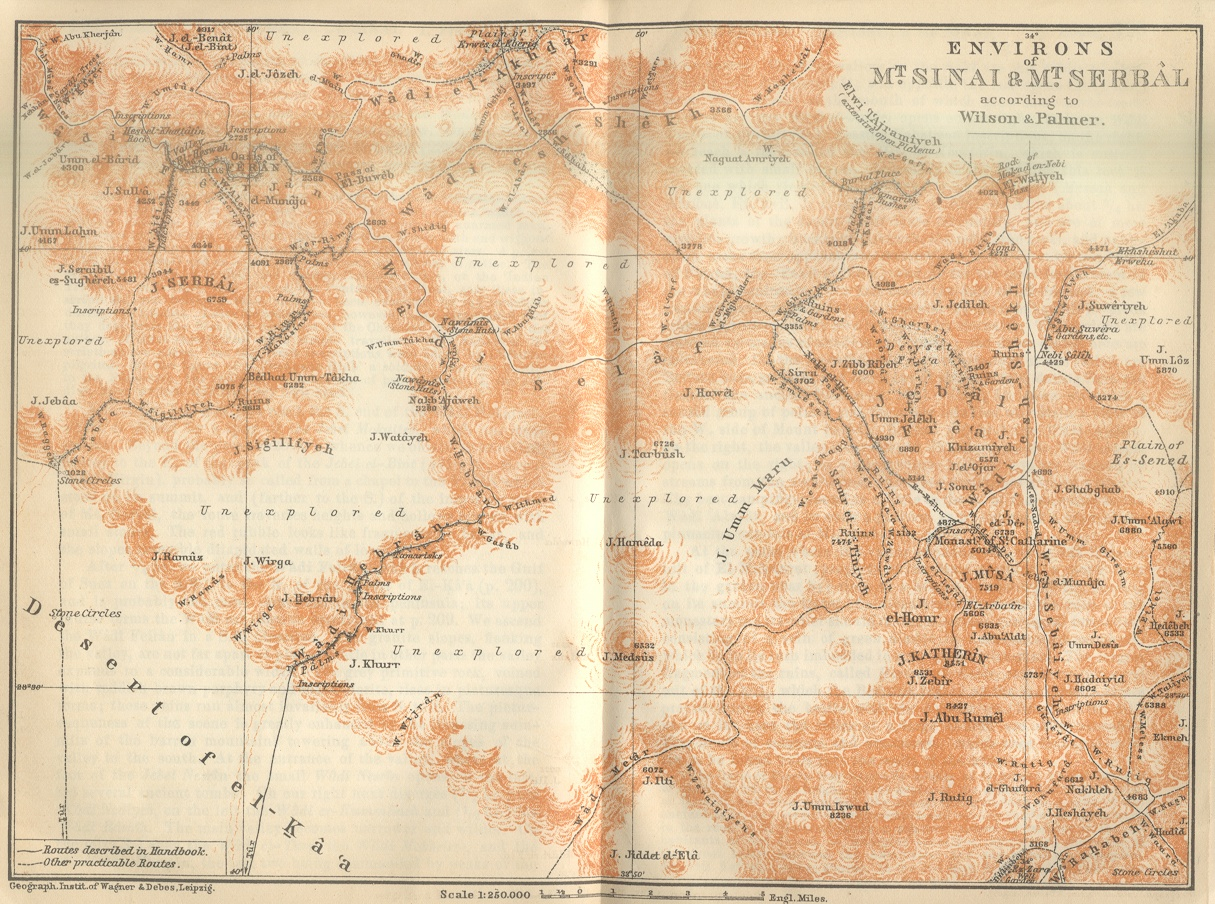
\includegraphics[clip,trim=5cm 2cm 9cm 1cm,width=\linewidth]{OldBookArt--MapImages-173.jpg}
\vfill
{\large \textit{This material is Open Game Content, and is licensed for public use under the terms of the Open Game License v1.0a.}\\
\today}
\end{center}

\pagebreak
\sffamily
\pagestyle{plain}
\raggedbottom

%%%%%%%%%%%%%%%%%%%%%%%%%%%%%%%%%%%%%%%%%%%%%%%%%%
%%%%%%%%%%%%%%%%%%%%%%%%%%%%%%%%%%%%%%%%%%%%%%%%%%
%%% Table of Contents
%%%%%%%%%%%%%%%%%%%%%%%%%%%%%%%%%%%%%%%%%%%%%%%%%%
%%%%%%%%%%%%%%%%%%%%%%%%%%%%%%%%%%%%%%%%%%%%%%%%%%
\renewcommand{\contentsname}{Table of Contents}
\setcounter{tocdepth}{1}
\tableofcontents

%%%%%%%%%%%%%%%%%%%%%%%%%%%%%%%%%%%%%%%%%%%%%%%%%%
%%%%%%%%%%%%%%%%%%%%%%%%%%%%%%%%%%%%%%%%%%%%%%%%%%
%%% Main Content
%%%%%%%%%%%%%%%%%%%%%%%%%%%%%%%%%%%%%%%%%%%%%%%%%%
%%%%%%%%%%%%%%%%%%%%%%%%%%%%%%%%%%%%%%%%%%%%%%%%%%

%% Primary Chapters Here

\clearpage

\chapter{Introduction}
\section{What is a Role-playing Game?}
foo
\section{What You Need To Play}
foo
\section{The Core Mechanic}
foo
\section{Creating a Character}
foo

\chapter{Races}
\section{Race Basics}
foo
\section{Drow}
foo
\section{Dwarf}
foo
\section{Elf}
foo
\section{Gnome}
foo
\section{Goblin}
foo
\section{Half-Elf}
foo
\section{Halfling}
foo
\section{Hobgoblin}
foo
\section{Human}
foo
\section{Kobold}
foo
\section{Orc}
foo

\chapter{Classes}
\section{Class Basics}
foo

\classname{Assassin} \label{class:assassin}
\vspace{-8pt}
\quot{"I kill people. Individually, you are a person. Collectively, I think you count as people."}

\desc{An assassin is a master of the art of killing, a vicious weapon honed by experience and inclination to learn the myriad ways to end a life. Unlike common warriors or rogues, an Assassin does not study various fighting arts or muddle his training with martial dirty tricks, he instead studies the anatomy of the various creatures of wildly different anatomies and forms of existence, and he uses this knowledge to place his blows in areas vital for biological or mystical reasons. Stealth and sudden violence are his hallmarks, and various exotic tools and killing methods become his tools.}

\desc{While most societies consider assassination to be a vile art, or at best a dishonorable or unvalorous one, the reasons that drive these killers vary. Cold-hearted mercenaries share a skill set with dedicated demon-hunters, differing only in the application of their skills. Only the most na\"ive student of ethics believes that all killing is evil, or that nobility cannot be found in a mercifully quick death.}

\ability{Alignment:}{An Assassin may be of any alignment.}

\ability{Races:}{Any}

\ability{Starting Gold:}{6d4x10 gp (150 gold)}

\ability{Starting Age:}{As Rogue.}

\ability{Hit Die:}{d6}

\ability{Class Skills:}{The Assassin's skills (and the key ability for each skill) are Balance (Dex), Bluff (Cha), Climb (Str), Concentration (Con), Craft (Int), Diplomacy (Cha), Disable Device (Int), Disguise (Cha), Gather Information (Cha), Hide (Dex), Intimidate (Cha), Jump (Str), Knowledge (all) (Int), Listen (Wis), Move Silently (Dex), Perform (Cha), Profession (Wis), Search (Int), Sense Motive (Wis), Sleight of Hand (Dex), Spellcraft (Int), Spot (Wis), Swim (Str), Tumble (Dex), and Use Magic Device (Cha).}

\ability{Skills/Level:}{6 + Intelligence Bonus}

\begin{table}[htb]
\begin{small}
\begin{tabular}{lp{1.9cm}p{0.7cm}p{0.7cm}p{0.7cm}l}
Level  &Base Attack Bonus &Fort Save &Ref Save &Will Save &Special\\
1st &+0 &+2 &+2 &+0 &Poison Use, Death Attack +3d6, Personal Immunity, Spellcasting\\
2nd &+1 &+3 &+3 &+0 &Uncanny Dodge, Death Attack +4d6\\
3rd &+2 &+3 &+3 &+1 &Hide in Plain Sight, Death Attack +5d6\\
4th &+3 &+4 &+4 &+1 &Cloak of Discretion, Death Attack +6d6\\
5th &+3 &+4 &+4 &+1 &Traps, Trapmaking, Death Attack +7d6\\
6th &+4 &+5 &+5 &+2 &Palm Weapon, Death Attack +8d6\\
7th &+5 &+5 &+5 &+2 &Full Death Attack, Death Attack +9d6\\
8th &+6/+1 &+6 &+6 &+2 &Nerve of the Assassin, Death Attack +10d6\\
9th &+6/+1 &+6 &+6 &+3 &Improved Uncanny Dodge, Death Attack +11d6\\
10th &+7/+2 &+7 &+7 &+3 &Skill Mastery, Death Attack +12d6\\
11th &+8/+3 &+7 &+7 &+3 &Poisonmaster, Death Attack +13d6\\
12th &+8/+3 &+8 &+8 &+4 &Personal Immunity, Death Attack +14d6\\
13th &+9/+4 &+8 &+8 &+4 &Exotic Method, Death Attack +15d6\\
14th &+10/+5 &+9 &+9 &+4 &Personal Immunity, Death Attack +16d6\\
15th &+11/+6/+6 &+9 &+9 &+5 &Killer's Proof, Death Attack +17d6\\
16th &+12/+7/+7 &+10 &+10 &+5 &Exotic Method, Death Attack +18d6\\
17th &+12/+7/+7 &+10 &+10 &+5 &Death by a Thousand Cuts, Death Attack +19d6\\
18th &+13/+8/+8 &+11 &+11 &+6 &Mind Blank, Death Attack +20d6\\
19th &+14/+9/+9 &+11 &+11 &+6 &Exotic Method, Death Attack +21d6\\
20th &+15/+10/+10 &+12 &+12 &+6 &Killing Strike, Death Attack +22d6\\
\end{tabular}
\end{small}
\end{table}

\begin{floatingfigure}{3.9in}
\begin{small}
\noindent\begin{tabular}{lllllllllllllllll}
 & \multicolumn{7}{c}{Assassin Spells Per Day}  &   &\multicolumn{7}{c}{Assassin Spells Known}\\
  &0 &1 &2 &3 &4 &5 &6 &  &  &0 &1 &2 &3 &4 &5 &6\\
1 &2 &- &- &- &- &- &- &  &1 &4 &- &- &- &- &- &-\\
2 &3 &0 &- &- &- &- &- &  &2 &5 &2 &- &- &- &- &-\\
3 &3 &1 &- &- &- &- &- &  &3 &6 &3 &- &- &- &- &-\\
4 &3 &2 &0 &- &- &- &- &  &4 &6 &3 &2 &- &- &- &-\\
5 &3 &3 &1 &- &- &- &- &  &5 &6 &4 &3 &- &- &- &-\\
6 &3 &3 &2 &- &- &- &- &  &6 &6 &4 &3 &- &- &- &-\\
7 &3 &3 &2 &0 &- &- &- &  &7 &6 &4 &4 &2 &- &- &-\\
8 &3 &3 &3 &1 &- &- &- &  &8 &6 &4 &4 &3 &- &- &-\\
9 &3 &3 &3 &2 &- &- &- &  &9 &6 &4 &4 &3 &- &- &-\\
10 &3 &3 &3 &2 &0 &- &- &  &10 &6 &4 &4 &4 &2 &- &-\\
11 &3 &3 &3 &3 &1 &- &- &  &11 &6 &4 &4 &4 &3 &- &-\\
12 &3 &3 &3 &3 &2 &- &- &  &12 &6 &4 &4 &4 &3 &- &-\\
13 &3 &3 &3 &3 &2 &0 &- &  &13 &6 &4 &4 &4 &4 &2 &-\\
14 &3 &3 &3 &3 &3 &1 &- &  &14 &6 &4 &4 &4 &4 &3 &-\\
15 &3 &3 &3 &3 &3 &2 &- &  &15 &6 &4 &4 &4 &4 &3 &-\\
16 &3 &3 &3 &3 &3 &2 &0 &  &16 &6 &5 &4 &4 &4 &4 &2\\
17 &3 &3 &3 &3 &3 &3 &1 &  &17 &6 &5 &5 &4 &4 &4 &3\\
18 &3 &3 &3 &3 &3 &3 &2 &  &18 &6 &5 &5 &5 &4 &4 &3\\
19 &3 &3 &3 &3 &3 &3 &3 &  &19 &6 &5 &5 &5 &5 &4 &4\\
20 &3 &3 &3 &3 &3 &3 &3 &  &20 &6 &5 &5 &5 &5 &5 &4\\
\end{tabular}
\end{small}
\end{floatingfigure}

\smallskip\noindent All of the following are Class Features of the Assassin class.

\ability{Weapon and Armor Proficiency:}{Assassins are proficient with all Light Weapons, as well as simple weapons, repeating crossbows, and hand crossbows. At first level, an Assassin gains proficiency with one Exotic Weapon of her choice. Assassins are proficient with Light Armor but not with shields.}

\ability{Spellcasting:}{The Assassin is an Arcane Spellcaster with the same spells per day and spells known progression as a Bard, except that he gains no more than three spell slots per level. An Assassin's spells known may be chosen from the Sorcerer/Wizard list, and must be from the schools of Divination, Illusion, or Necromancy. To cast an Assassin spell, she must have an Intelligence at least equal to 10 + the Spell level. The DC of the Assassin's spells is Intelligence based and the bonus spells are Intelligence based.}

\ability{Poison Use (Ex):}{An Assassin may prepare, apply, and use poison without any chance of poisoning herself.}

\ability{Death Attack (Ex):}{An Assassin may spend a full-round action to study an opponent who would be denied their Dexterity bonus if she instead attacked that target. If she does so, her next attack is a Death Attack if she makes it within 1 round. A Death Attack inflicts a number of extra dice of damage equal to her Assassin level plus two dice, but only if the target is denied its Dexterity Bonus to AC against that attack. Special attacks such as a coup de grace may be a Death Attack. Assassins are well trained in eliminating magical or distant opponents, and do not have to meet the stringent requirements of a sneak attack, though if a character has both sneak attack and death attack, they stack if the character meets the requirements of both. As long as the victim is denied their dexterity against attacks from the assassin during the study action and the attack itself, it counts as a death attack. An Assassin may load a crossbow simultaneously with his action to study his target if he has a Base Attack Bonus of +1 or more.}

\ability{Personal Immunity (Ex):}{Choose four poisons, an Assassin is immune to all four of those poisons, even if they are made available in a stronger strength. At levels 5, 7, and 12 the Assassin may choose one more type of poison to become immune to. At level 14, an Assassin becomes immune to all poisons.}

\ability{Uncanny Dodge (Ex):}{Starting at 2nd level, an Assassin can react to danger before his senses would normally allow him to do so. He retains her Dexterity bonus to AC (if any) even if she is caught flat-footed or struck by an invisible attacker. However, he still loses her Dexterity bonus to AC if immobilized. If an Assassin already has uncanny dodge from a different class he automatically gains improved uncanny dodge (see below) instead.}

\ability{Hide in Plain Sight (Ex):}{A 3rd level Assassin can hide in unusual locations, and may hide in areas without cover or concealment without penalty. An Assassin may even hide while being observed. This ability does not remove the -10 penalty for moving at full speed, or the -20 penalty for running or fighting.}

\ability{Cloak of Discretion (Su):}{At 4th level, an Assassin is protected by a constant \emph{nondetection} effect, with a caster level equal to his character level.}

\ability{Trapfinding:}{At 5th level, Assassins can use the Search skill to locate traps when the task has a Difficulty Class higher than 20. Finding a nonmagical trap has a DC of at least 20, or higher if it is well hidden. Finding a magic trap has a DC of 25 + the level of the spell used to create it. Assassins can use the Disable Device skill to disarm magic traps. A magic trap generally has a DC of 25 + the level of the spell used to create it. An Assassin who beats a trap's DC by 10 or more with a Disable Device check can study a trap, figure out how it works, and bypass it (with her party) without disarming it.}

\ability{Trapmaking:}{At 5th level, the Assassin learns to build simple mechanical traps in out of common materials. As long as has access to ropes, flexible material like green wood, and weapon-grade materials like sharpened wooden sticks or steel weapons, he can build an improvised trap in 10 minutes. He can build any non-magical trap on the "CR 1" trap list that doesn't involve a pit. These traps have a Search DC equal to 20 + the Assassin's level, have a BAB equal to his own, and are always single-use traps. He may add poison to these traps, if he has access to it, but it will dry out in an hour.}

\ability{Palm Weapon (Su):}{At 6th level, the Assassin learns to conceal weapons with supernatural skill. Any weapon successfully concealed with Sleight of Hand cannot be found with divination magic.}

\ability{Full Death Attack:}{At 7th level, if the Assassin studies an opponent to perform a Death Attack, she can make a full attack during the next round where every attack inflicts Death Attack damage as long as the target was denied their Dexterity bonus to AC against the first attack in the full attack action.}

\ability{Nerve of the Killer:}{At 8th level, an Assassin gains a limited immunity to compulsion and charm effects. While studying a target for a Death Attack, and for one round afterward, he counts as if he were within a \spell{protection from evil} effect. This does not confer a deflection bonus to AC.}

\ability{Improved Uncanny Dodge (Ex):}{An Assassin of 9th level or higher can no longer be flanked. This defense denies another character the ability to sneak attack the character by flanking him, unless the attacker has at least four more levels in a class that provides sneak attack than the target. If a character already has uncanny dodge (see above) from a second class, the character automatically gains improved uncanny dodge instead, and the levels from the classes that grant uncanny dodge stack to determine the minimum level required to flank the character.}

\ability{Skill Mastery (Ex):}{At 10th level, an Assassin becomes so certain in the use of certain skills that she can use them reliably even under adverse conditions. When making a skill check with Climb, Disable Device, Hide, Move Silently, Search, Spellcraft, Use Magic Device, Use Rope, or Swim, she may take 10 even if stress and distractions would normally prevent her from doing so.}

\ability{Poisonmaster:}{At 11th level, the Assassin learns alchemic secrets for creating short-term poisons. By expending an entire healer's kit worth of materials and an hour of time, he can synthesize one dose of any poison in the DMG. This poison degrades to uselessness in one week.}

\ability{Exotic Method:}{At 13th, 16th, and 19th level the Assassin learns an exotic form of killing from the list below. Once chosen, this ability does not change:}
\listone

    \item \ability{Carrier:}{Three times per day, the Assassin can cast \spell{contagion} as a swift action spell-like ability.}
    \item \ability{Poison of the Cockatrice:}{Twice per day, the Assassin can cast \spell{flesh to stone} as a swift action spell-like ability.}
    \item \ability{Killer Faerie Arts:}{Twice per day, the Assassin can cast \spell{polymorph other} as a swift action spell-like ability.}
    \item \ability{Proxy Assassin:}{Twice per day, the Assassin can cast \spell{summon monster VII} as a spell-like ability. This effect lasts 10 minutes.}
    \item \ability{Death By Plane:}{Once per day, the Assassin can cast \spell{plane shift} as a spell-like ability.}
    \item \ability{Dimesional Rip:}{Once per day, the Assassin can cast \spell{implosion} as a spell-like ability. The duration of this effect is three rounds.}
    \item \ability{New School:}{The Assassin may now choose spells known from a new school.}
\end{list}
\vspace{8pt}

\ability{Killer's Proof (Su):}{At 15th level, the Assassin learns to steal the souls of those he kills. If he is holding an onyx worth at least 100 GP when he kills an enemy, he may place their soul within the gem as if he has cast \spell{soul bind} on them at the moment of their death.}

\ability{Death by a Thousand Cuts:}{At 17th level, the assassin has learned to kill even the hardiest of foes by reducing their physical form to shambles. Every successful Death attack inflicts a cumulative -2 Dexterity penalty to the Assassin's victim. These penalties last one day.}

\ability{Mind Blank (Su):}{At 18th level, the Assassin is protected by a constant \spell{mind blank} effect.}

\ability{Killing Strike (Su):}{At 20th level, the Assassin's Death Attacks bypass his victim's DR and hardness.}

\section{Barbarian}
foo
\section{Bard}
foo
\section{Cleric}
foo
\section{Druid}
foo
\section{Fighter}
foo
\section{Knight}
foo
\section{Monk}
foo
\section{Paladin}
foo
\section{Ranger}
foo
\section{Rogue}
foo
\section{Samurai}
foo
\section{Sorcerer}
foo
\section{Wizard}
foo

\chapter{Skills}
\section{How Skills Work}
foo
\section{Appraise}
foo
\section{Athletics}
foo
\section{Balance}
foo
\section{Bluff}
foo
\section{Concentration}
foo
\section{Craft}
foo
\section{Decipher Script}
foo
\section{Diplomacy}
foo
\section{Disable Device}
foo
\section{Disguise}
foo
\section{Escape Artist}
foo
\section{Forgery}
foo
\section{Gather Information}
foo
\section{Handle Animal}
foo
\section{Heal}
foo
\section{Intimidate}
foo
\section{Knowledge}
foo
\section{Perception}
foo
\section{Perform}
foo
\section{Profession}
foo
\section{Ride}
foo
\section{Search}
foo
\section{Sense Motive}
foo
\section{Sleight of Hand}
foo
\section{Speak Language}
foo
\section{Spellcraft}
foo
\section{Stealth}
foo
\section{Survival}
foo
\section{Tumble}
foo
\section{Use Magic Device}
foo

\chapter{Feats}
\section{How Feats Work}
foo
\section{General Feats}
foo
\section{Combat Feats}
foo
\section{Skill Feats}
foo
\section{Metamagic Feats}
foo

\chapter{Goods and Services}
\section{The Three Economies}
foo
\section{Armor}
foo
\section{Weapons}
\section{Weapons}
\vspace*{-10pt}
\quot{''No. This is a knife."}


The weapon system of D\&D, in general, makes us feel pretty good. There are ample reasons to use weapons as diverse as a flail, a warhammer, and a morningstar. There are, however, some glaring problems that do need to be addressed. The most obvious of those is Weapon Size, which works very badly on every level. The 3rd edition rules were not good, and the 3.5 changes to them made them worse in every single way. So here's the big deal: Weapons don't have special size rules anymore. In 3rd edition a Shortsword was a small weapon, and in 3.5 it's supposed to be a Medium Light Weapon, but that's all stupid. The fact is, a Shortsword is a Tiny Object, and that's all we need to know.

Here's how weapon sizes ought to work:

\listone
    \item You may not use a weapon that is a larger than yourself. A Large character can use a Large (or smaller) object as a weapon, but may not use a Huge (or larger) object as a weapon.
    \item You may not use an object that is too heavy for you to lift as a light load as a weapon.
    \item An object of your own size must be used in two hands.
    \item An object of a size smaller than your size may be used in one hand or two hands.
    \item An object that is at least two sizes smaller than yourself counts as a Light Weapon.
\end{list}


\subsection{Bows}

The bow is a very expensive proposition in the normal D\&D rules. Especially for Orcs. That's really dumb. So here are the new rules:

Every bow has a strength minimum. And it doesn't cost any more if it has a Strength Minimum of 34 than it does if it has a Strength minimum of 6. In any case, your bow can't be used if your strength is less than the strength minimum of the bow. But, your bow does damage based on your actual strength -- or 4 more than the strength minimum of the bow, whichever is less.

Now, certain groups are not going to have bows available with a strength bonus applicable to yourself. If you have a strength of 8, the Bugbears probably won't have any bows off the shelf to sell to you. If you have a strength of 18, the Kobolds won't have anything for you. If you're in an area that doesn't normally make bows for you, you're going to have to get a masterwork bow made for you -- and that costs extra moneys.

Now, the range of a bow is based on its object size. A Medium object (the kind of bow you are most likely to use) has a range increment of 100 feet. Every size it is smaller than that decreases the range increment by 30 feet (yes, that means that Fine creatures don't even have bows, and we're OK with that). Every size that a bow is larger than medium increases the range increment by 30 feet. A composite bow has an extra 10 feet of range increment. A character may only use a composite bow or a bow that is smaller than herself while mounted. And yes, a bow is two handed even if it is an object two sizes smaller than yourself.

\subsection{Ammunition}
\vspace*{-8pt}
\quot{''The Black Arrow was forged by Thror the Dwarf, who was ''King Under The (Lonely) Mountain," and ultimately was destroyed when Bard used it for target practice against a swallow, thereby dooming most of Middle Earth."}

The ammunition rules are in need of adjustment. And that's not just because having a shuriken get destroyed permanently every time it hits is really dumb. It's almost balanced to have magic arrows cost about 1/50th of what a real magic weapon does and then explode when used like they were bullets or something. Almost. But it is also dumb, so we're putting our foot down.

Magic Arrows are supposed to be awesome. Some of them even have names. I cannot recall any story where an insipid adventurer went to War with 137 magic arrows and then called it a day when every one of them had been fired once. So here's the new rubric: the cost of enchanting a magical arrow is a mere 1/10th that of enchanting a weapon (move the decimal place over one place), and magical arrows are always recoverable. That's part of what makes them magic. Of course, just because it's recoverable, doesn't mean that you will actually recover it. If you shoot three arrows into a guy and then you run away, chances are good that he has your arrow.

Heck, even regular ammunition is way too fragile in D\&D. Shuriken are fairly reusable even after you pull them out of the eye of a fallen foe. And we're fine with that. A good rule of thumb is that an item of ammunition is no longer usable if it inflicts more damage that it has hardness. And precision damage, such as Sneak Attack, Death Attack, and Sudden Strike, does not count. So yeah, Shuriken aren't going to break on impact with small children, happy birthday.

Naturally enough, there are still one-use arrows in the world. Alchemical arrows, such as fire arrows or poison arrows, are generally not as useful after they've been shot into an appropriate target. Those don't require magical forging however, and don't really count as magic weapons. One use ranged weapons should be marked as such (such as the vial of acid, hard to reuse that one).

\subsection{Necromatic Weapons}

\listone
\itemability{Boneblades:} Boneblades are alchemically and necromantically hardened blades made from the bones of intelligent creatures, and the material can only be created by craftsmen with the Boneblade Master feat. For an unknown reason, they only retain their special properties if they are made into light slashing or piercing weapons.

Boneblades used in melee combat ignore the damage reduction of any undead creature and can hit incorporeal creatures as if they were magic weapons with the ghost touch property.

Boneblades made from dragon bones can be combined with the Dragoncrafter feat to produce items with both properties.

Cost: 1,000 gp per lb.

\itemability{Blood Steel:} Blood steel is steel that has been mixed with the blood of certain powerful creatures, making it redder than normal steel and with unusual properties.

Weapons made of blood steel do 2 additional points of damage on a successful hit.

Cost: 2,000 gp for a weapon

\itemability{Black Steel:} Black steel is steel that has been mixed with necromantically charged obsidian, making it as sharp as adamantine and as dangerous as obsidian. Weapons made of black steel count as adamantine for all effects, but perform as if enhanced with the Ghost Touch and Wounding properties (without additional cost).

Characters using items made of black steel suffer one point of Wisdom drain for every day they are held, worn or carried.

Cost: 15,000 gp for a weapon  %, 24,000 gp for light armor, 28,000 gp for medium armor, 32,000 gp for heavy armor.\\

\end{list} 

\section{Gear}
foo
\section{Animals}
foo
\section{Services}
foo

\chapter{Description}
\section{Physical Appearance}
foo
\section{Personality}
foo
\section{Alignment}
foo
\section{Religion}
foo

\chapter{Adventuring}
\section{Overland Travel}
foo
\section{Exploration}
foo
\section{Traps}
foo
\section{Encounters}
foo

\chapter{Combat}
\section{How Combat Works}
foo
\section{Combat Statistics}
foo
\section{Initiative and Actions}
foo
\section{Standard Actions}
foo
\section{Move Actions}
foo
\section{Swift and Free Actions}
foo
\section{Full-Round Actions}
foo
\section{Movement, Position, and Distance}
foo
\section{Injury and Death}
foo
\section{Combat Modifiers}
foo
\section{Special Attacks}
foo
\section{Special Abilities}
foo
\section{Conditions}
foo

\chapter{Magic}
\section{Casting Spells}
foo
\section{How To Read A Spell Description}
foo
\section{Arcane Spells}
foo
\section{Divine Spells}
foo
\section{Special Abilities and Spells}
foo
\section{Spell Lists}
foo

\chapter{Magic Items}
\section{Magic Item Basics}
Scaling, 8 Item Limit, etc
\section{Minor Magical Items}
foo
\section{Moderate Magical Items}
foo
\section{Major Magical Items}
foo

\chapter{Running The Game}
\section{Writing GM Advice Is Hard}
foo

%%%%%%%%%%%%%%%%%%%%%%%%%%%%%%%%%%%%%%%%%%%%%%%%%%
%%%%%%%%%%%%%%%%%%%%%%%%%%%%%%%%%%%%%%%%%%%%%%%%%%
\appendix
%%%%%%%%%%%%%%%%%%%%%%%%%%%%%%%%%%%%%%%%%%%%%%%%%%
%%%%%%%%%%%%%%%%%%%%%%%%%%%%%%%%%%%%%%%%%%%%%%%%%%
\appendixpage

\makeatletter
\renewcommand{\@makechapterhead}[1]{%
\vspace*{0 pt}{
\raggedright \normalfont \fontsize{32}{32} \selectfont \bfseries
\ifnum \value{secnumdepth}>-1
  \if@mainmatter \vspace{-8pt} {\fontsize{20}{20} \selectfont Appendix \thechapter:}\\[8pt]
  \fi%
\fi
\hspace{0.65cm} #1\par\nobreak\vspace{20 pt}
}}
\makeatother

\clearpage

%% Appendix Chapters Here

\chapter{Spells}
\section{Spells, A through Z}
foo

\chapter{Prestige Classes}
\section{Prestige Class Basics}
\section{?WhatClasses?}

\chapter{Monsters}
\section{Reading a Monster Entry}
\section{Monsters, A though Z}

\chapter{NPC Classes}
\section{Adept}
\section{Aristocrat}
\section{Commoner}
\section{Expert}
\section{Warrior}

%%%%%%%%%%%%%%%%%%%%%%%%%%%%%%%%%%%%%%%%%%%%%%%%%%
%%%%%%%%%%%%%%%%%%%%%%%%%%%%%%%%%%%%%%%%%%%%%%%%%%
\chapter{The Open Game License}
%%%%%%%%%%%%%%%%%%%%%%%%%%%%%%%%%%%%%%%%%%%%%%%%%%
%%%%%%%%%%%%%%%%%%%%%%%%%%%%%%%%%%%%%%%%%%%%%%%%%%
\label{Open Game License}

The text and tables of this document are Open Game Content as defined in the Open Game License below. The images of this document are Product Identity. You can compare this work to any other work that you like in any way.

Images within this document are not released under the OGL. Instead they are used under a \href{http://creativecommons.org/licenses/by-sa/3.0/}{Creative Commons Attribution-ShareAlike} license, and come from the following sources:
\begin{description*}
\item[Cover Image] \href{http://www.gallery.oldbookart.com/main.php?g2_itemId=10682}{Courtesy of OldBookArt.com}
\end{description*}

\oldsection*{OPEN GAME LICENSE Version 1.0a}

\begin{small}

The following text is the property of Wizards of the Coast, Inc. and is Copyright 2000 Wizards of the Coast, Inc ("Wizards"). All Rights Reserved.

\begin{enumerate}\raggedright
\item \textbf{Definitions}:
	\begin{enumerate}[(a)]\raggedright
	\item "Contributors" means the copyright and/or trademark owners who have contributed Open Game Content;
	\item "Derivative Material" means copyrighted material including derivative works and translations (including into other computer languages), potation, modification, correction, addition, extension, upgrade, improvement, compilation, abridgment or other form in which an existing work may be recast, transformed or adapted;
	\item "Distribute" means to reproduce, license, rent, lease, sell, broadcast, publicly display, transmit or otherwise distribute;
	\item "Open Game Content" means the game mechanic and includes the methods, procedures, processes and routines to the extent such content does not embody the Product Identity and is an enhancement over the prior art and any additional content clearly identified as Open Game Content by the Contributor, and means any work covered by this License, including translations and derivative works under copyright law, but specifically excludes Product Identity.
	\item "Product Identity" means product and product line names, logos and identifying marks including trade dress; artifacts; creatures characters; stories, storylines, plots, thematic elements, dialogue, incidents, language, artwork, symbols, designs, depictions, likenesses, formats, poses, concepts, themes and graphic, photographic and other visual or audio representations; names and descriptions of characters, spells, enchantments, personalities, teams, personas, likenesses and special abilities; places, locations, environments, creatures, equipment, magical or supernatural abilities or effects, logos, symbols, or graphic designs; and any other trademark or registered trademark clearly identified as Product identity by the owner of the Product Identity, and which specifically excludes the Open Game Content;
	\item "Trademark" means the logos, names, mark, sign, motto, designs that are used by a Contributor to identify itself or its products or the associated products contributed to the Open Game License by the Contributor
	\item "Use", "Used" or "Using" means to use, Distribute, copy, edit, format, modify, translate and otherwise create Derivative Material of Open Game Content.
	\item "You" or "Your" means the licensee in terms of this agreement.
	\end{enumerate}

\item \textbf{The License}: This License applies to any Open Game Content that contains a notice indicating that the Open Game Content may only be Used under and in terms of this License. You must affix such a notice to any Open Game Content that you Use. No terms may be added to or subtracted from this License except as described by the License itself. No other terms or conditions may be applied to any Open Game Content distributed using this License. 

\item \textbf{Offer and Acceptance}: By Using the Open Game Content You indicate Your acceptance of the terms of this License. 

\item \textbf{Grant and Consideration}: In consideration for agreeing to use this License, the Contributors grant You a perpetual, worldwide, royalty-free, non-exclusive license with the exact terms of this License to Use, the Open Game Content. 

\item \textbf{Representation of Authority to Contribute}: If You are contributing original material as Open Game Content, You represent that Your Contributions are Your original creation and/or You have sufficient rights to grant the rights conveyed by this License. 

\item \textbf{Notice of License Copyright}: You must update the COPYRIGHT NOTICE portion of this License to include the exact text of the COPYRIGHT NOTICE of any Open Game Content You are copying, modifying or distributing, and You must add the title, the copyright date, and the copyright holder's name to the COPYRIGHT NOTICE of any original Open Game Content you Distribute. 

\item \textbf{Use of Product Identity}: You agree not to Use any Product Identity, including as an indication as to compatibility, except as expressly licensed in another, independent Agreement with the owner of each element of that Product Identity. You agree not to indicate compatibility or co-adaptability with any Trademark or Registered Trademark in conjunction with a work containing Open Game Content except as expressly licensed in another, independent Agreement with the owner of such Trademark or Registered Trademark. The use of any Product Identity in Open Game Content does not constitute a challenge to the ownership of that Product Identity. The owner of any Product Identity used in Open Game Content shall retain all rights, title and interest in and to that Product Identity. 

\item \textbf{Identification}: If you distribute Open Game Content You must clearly indicate which portions of the work that you are distributing are Open Game Content. 

\item \textbf{Updating the License}: Wizards or its designated Agents may publish updated versions of this License. You may use any authorized version of this License to copy, modify and distribute any Open Game Content originally distributed under any version of this License. 

\item \textbf{Copy of this License}: You MUST include a copy of this License with every copy of the Open Game Content You Distribute. 

\item \textbf{Use of Contributor Credits}: You may not market or advertise the Open Game Content using the name of any Contributor unless You have written permission from the Contributor to do so. 

\item \textbf{Inability to Comply}: If it is impossible for You to comply with any of the terms of this License with respect to some or all of the Open Game Content due to statute, judicial order, or governmental regulation then You may not Use any Open Game Material so affected. 

\item \textbf{Termination}: This License will terminate automatically if You fail to comply with all terms herein and fail to cure such breach within 30 days of becoming aware of the breach. All sublicenses shall survive the termination of this License. 

\item \textbf{Reformation}: If any provision of this License is held to be unenforceable, such provision shall be reformed only to the extent necessary to make it enforceable. 

\item \textbf{COPYRIGHT NOTICE}

\href{http://www.wizards.com/default.asp?x=d20/oglfaq/20040123f}{\textit{Open Game License v 1.0a}} Copyright 2000, Wizards of the Coast, Inc. 

\href{http://www.wizards.com/default.asp?x=d20/article/srd35}{\textit{System Reference Document}} Copyright 2000-2003, Wizards of the Coast, Inc.; Authors Jonathan Tweet, Monte Cook, Skip Williams, Rich Baker, Andy Collins, David Noonan, Rich Redman, Bruce R. Cordell, John D. Rateliff, Thomas Reid, James Wyatt, based on original material by E. Gary Gygax and Dave Arneson.

\href{http://www.tgdmb.com/viewtopic.php?t=34248}{\textit{Tome of Necromancy}} Copyright 2006, Frank Trollman and K

\href{http://www.tgdmb.com/viewtopic.php?t=28828}{\textit{Tome of Fiends}} Copyright 2006, Frank Trollman and K

\href{http://www.tgdmb.com/viewtopic.php?t=28547}{\textit{Dungeonomicon}} Copyright 2006, Frank Trollman and K

\href{http://www.tgdmb.com/viewtopic.php?t=33294}{\textit{Races of War}} Copyright 2006, Frank Trollman and K

\href{http://www.tgdmb.com/viewtopic.php?t=35813}{\textit{Book of Gears}} Copyright 2007, Frank Trollman and K

\href{https://github.com/SqueeG/awesomeTome}{\textit{Tome Reference Document}} Copyright 2013, Daniel Gee, ExplosiveRunes, SqueeG, and Tarkisflux
\end{enumerate}

END OF LICENSE

\end{small}

\clearpage
\phantomsection
\listoftables

\clearpage
\phantomsection
\printindex

\end{document}